\section{Berkeley-Adobe Perceptual Patch Similarity (BAPPS) Dataset}
\label{sec:methods}

To evaluate the performance of different perceptual metrics, we collect a large-scale highly diverse dataset of perceptual judgments using two approaches.
Our main data collection employs a two alternative forced choice (2AFC) test, that asks which of two distortions is more similar to a reference.
This is validated by a second experiment where we perform a just noticeable difference (JND) test, which asks whether two patches -- one reference and one distorted -- are the same or different. These judgments are collected over a wide space of distortions and real algorithm outputs.

\subfile{tables/pert}

\subsection{Distortions}

\paragraph{Traditional distortions} We create a set of ``traditional" distortions consisting of common operations performed on the input patches, listed in Table~\ref{tab:distortions} (left). In general, we use photometric distortions, random noise, blurring, spatial shifts and corruptions, and compression artifacts. We show qualitative examples of our traditional distortions in Figure \ref{fig:pert}. The severity of each perturbation is parameterized - for example, for Gaussian blur, the kernel width determines the amount of corruption applied to the input image. We also compose pairs of distortions sequentially to increase the overall space of possible distortions. In total, we have 20 distortions and 308 sequentially composed distortions.

\paragraph{CNN-based distortions} To more closely simulate the space of artifacts that can arise from deep-learning based methods, we create a set of distortions created by neural networks. We simulate possible algorithm outputs by exploring a variety of tasks, architectures, and losses, as shown in Table \ref{tab:distortions} (right). Such tasks include autoencoding, denoising, colorization, and superresolution. All of these tasks can be achieved by applying the appropriate corruption to the input. In total, we generated 96 ``denoising autoencoders" and use these as CNN-based distortion functions. We train each of these  networks on the 1.3M ImageNet dataset~\cite{russakovsky2015imagenet} for 1 epoch. The goal of each network is not to solve the task per se, but rather to explore common artifacts that plague the outputs of deep learning based methods.

\paragraph{Distorted image patches from real algorithms}
The true test of an image assessment algorithm is on real problems and real algorithms. 
We gather perceptual judgments using such outputs. Data on real algorithms is more limited, as each application will have their own unique properties. For example, different colorization methods will not show much structural variation, but will be prone to effects such as color bleeding and color variation. On the other hand, superresolution will not have color ambiguity, but may see larger structural changes from algorithm to algorithm.

\paragraph{Superresolution} We evaluate results from the 2017 NTIRE workshop~\cite{Agustsson_2017_CVPR_Workshops}. We use 3 tracks from the workshop -- $\times2$, $\times3$, $\times4$ upsampling rates using ``unknown" downsampling to create the input images. Each track had approximately 20 algorithm submissions. We also evaluate several additional methods, including bicubic upsampling, and four of the top performing deep superresolution methods~\cite{kim2016accurate,wang2015deep,ledig2016photo,sajjadi2016enhancenet}. A common qualitative way of presenting superresolution results is zooming into specific patches and comparing differences. As such, we sample random $64\times 64$ triplets from random locations of images in the Div2K~\cite{Agustsson_2017_CVPR_Workshops} dataset -- the ground truth high-resolution image, along with two algorithm outputs.

\paragraph{Frame interpolation} We sample patches from different frame interpolation algorithms, including three variants of flow-based interpolation~\cite{liu2009beyond}, CNN-based interpolation~\cite{Niklaus_ICCV_2017}, and phase-based interpolation~\cite{meyer2015phase} on the Davis Middleburry dataset~\cite{scharstein2002taxonomy}. Because artifacts arising from frame interpolation may occur at different scales, we randomly rescale the image before sampling a patch triplet.

\paragraph{Video deblurring} We sample from the video deblurring dataset~\cite{Su_2017_CVPR}, along with deblurring outputs from Photoshop Shake Reduction, Weighted Fourier Aggregation~\cite{delbracio2015hand}, and three variants of a deep video deblurring method~\cite{Su_2017_CVPR}.

\paragraph{Colorization} We sample patches using random scales on the colorization task, on images from the ImageNet dataset~\cite{russakovsky2015imagenet}. The algorithms are from pix2pix~\cite{isola2015learning}, Larsson et al.~\cite{larsson2016learning}, and variants from Zhang et al.~\cite{zhang2016colorful}.

\subsection{Psychophysical Similarity Measurements}

\paragraph{2AFC similarity judgments}
We randomly select an image patch $x$ and apply two distortions to produce patches $x_0, x_1$. We then ask a human which is closer to the original patch $x$, and record response $h \in \{0,1\}$. On average, people spent approximately 3 seconds per judgment. Let $\mathcal{T}$ denote our dataset of patch triplets $(x, x_0, x_1, h)$.

A comparison between our dataset and previous datasets is shown in Table~\ref{tab:dataset_comp}. 
Previous datasets have focused on collecting large numbers of human judgments for a few images and distortion types. 
For example, the largest dataset, TID2013~\cite{ponomarenko2015image}, has 500k judgments on 3000 distortions (from 25 input images with 24 distortions types, each sampled at 5 levels). 
We provide a complementary dataset that focuses instead on a large number of distortions types. In, addition, we collect judgments on a large number of $64\times 64$ patches rather than a small number of images.
There are three reasons for this. 
First, the space of full images is extremely large, which makes it much harder to cover a reasonable portion of the domain with judgments (even $64\times 64$ color patches represent an intractable 12k-dimensional space).
Second, by choosing a smaller patch size, we focus on lower-level aspects of similarity, to mitigate the effect of differing ``respects of similarity" that may be influenced by high-level semantics \cite{medin1993respects}. Finally, modern methods for image synthesis train deep networks with patch-based losses (implemented as convolutions)~\cite{chen2017photographic,isola2017image}. 
Our dataset consists of over 161k patches, derived from the MIT-Adobe 5k dataset~\cite{fivek} (5000 uncompressed images) for training, and the RAISE1k dataset~\cite{dang2015raise} for validation.

To enable large-scale collection, our data is collected ``in-the-wild" on Amazon Mechanical Turk, as opposed to a controlled lab setting. 
Crump et al.~\cite{crump2013evaluating} show that AMT can be reliably used to replicate many psychophysics studies, despite the inability to control all environmental factors.
We ask for 2 judgments per example in our ``train" set and 5 judgments in our ``val" sets.
Asking for fewer judgments enables us to explore a larger set of image patches and distortions. We add sentinels which consist of pairs of patches with obvious deformations, e.g., a large amount of Gaussian noise vs a small amount of Gaussian noise. Approximately $~90\%$ of Turkers were able to correctly pass at least $93\%$ of the sentinels (14 of 15), indicating that they understood the task and were paying attention.
We choose to use a larger number of distortions than prior datasets.

\subfile{tables/dataset_split}

\paragraph{Just noticeable differences (JND)}

A potential shortcoming of the 2AFC task is that it is ``cognitively penetrable," in the sense that participants can consciously choose which respects of similarity they will choose to focus on in completing the task \cite{medin1993respects}, which introduces subjectivity into the judgments. To validate that the judgments actually reflected something objective and meaningful, we also collected user judgments of ``just noticeable differences" (JNDs). We show a reference image, followed by a randomly distorted image, and ask a human if the images are the same or different.
The two image patches are shown for 1 second each, with a 250 ms gap in between. 
Two images which look similar may be easily confused, and a good perceptual metric will be able to order pairs from most to least confusable. 
JND tests like this may be considered less subjective, since there is a single correct answer for each judgment, and participants are presumed to be aware of what correct behavior entails. We gather 3 JND observations for each of the 4.8k patches in our traditional and CNN-based validation sets. 
Each subject is shown 160 pairs, along with 40 sentinels (32 identical and 8 with large Gaussian noise distortion applied).
We also provide a short training period of 10 pairs which contain 4 ``same" pairs, 1 obviously different pair, and 5 ``different" pairs generated by our distortions. 
We chose to do this in order to prime the users towards expecting approximately $40\%$ of the patch pairs to be identical. 
Indeed, $36.4\%$ of the pairs were marked ``same" ($70.4\%$ of sentinels and $27.9\%$ of test pairs).

\begin{figure*}
  \centering
  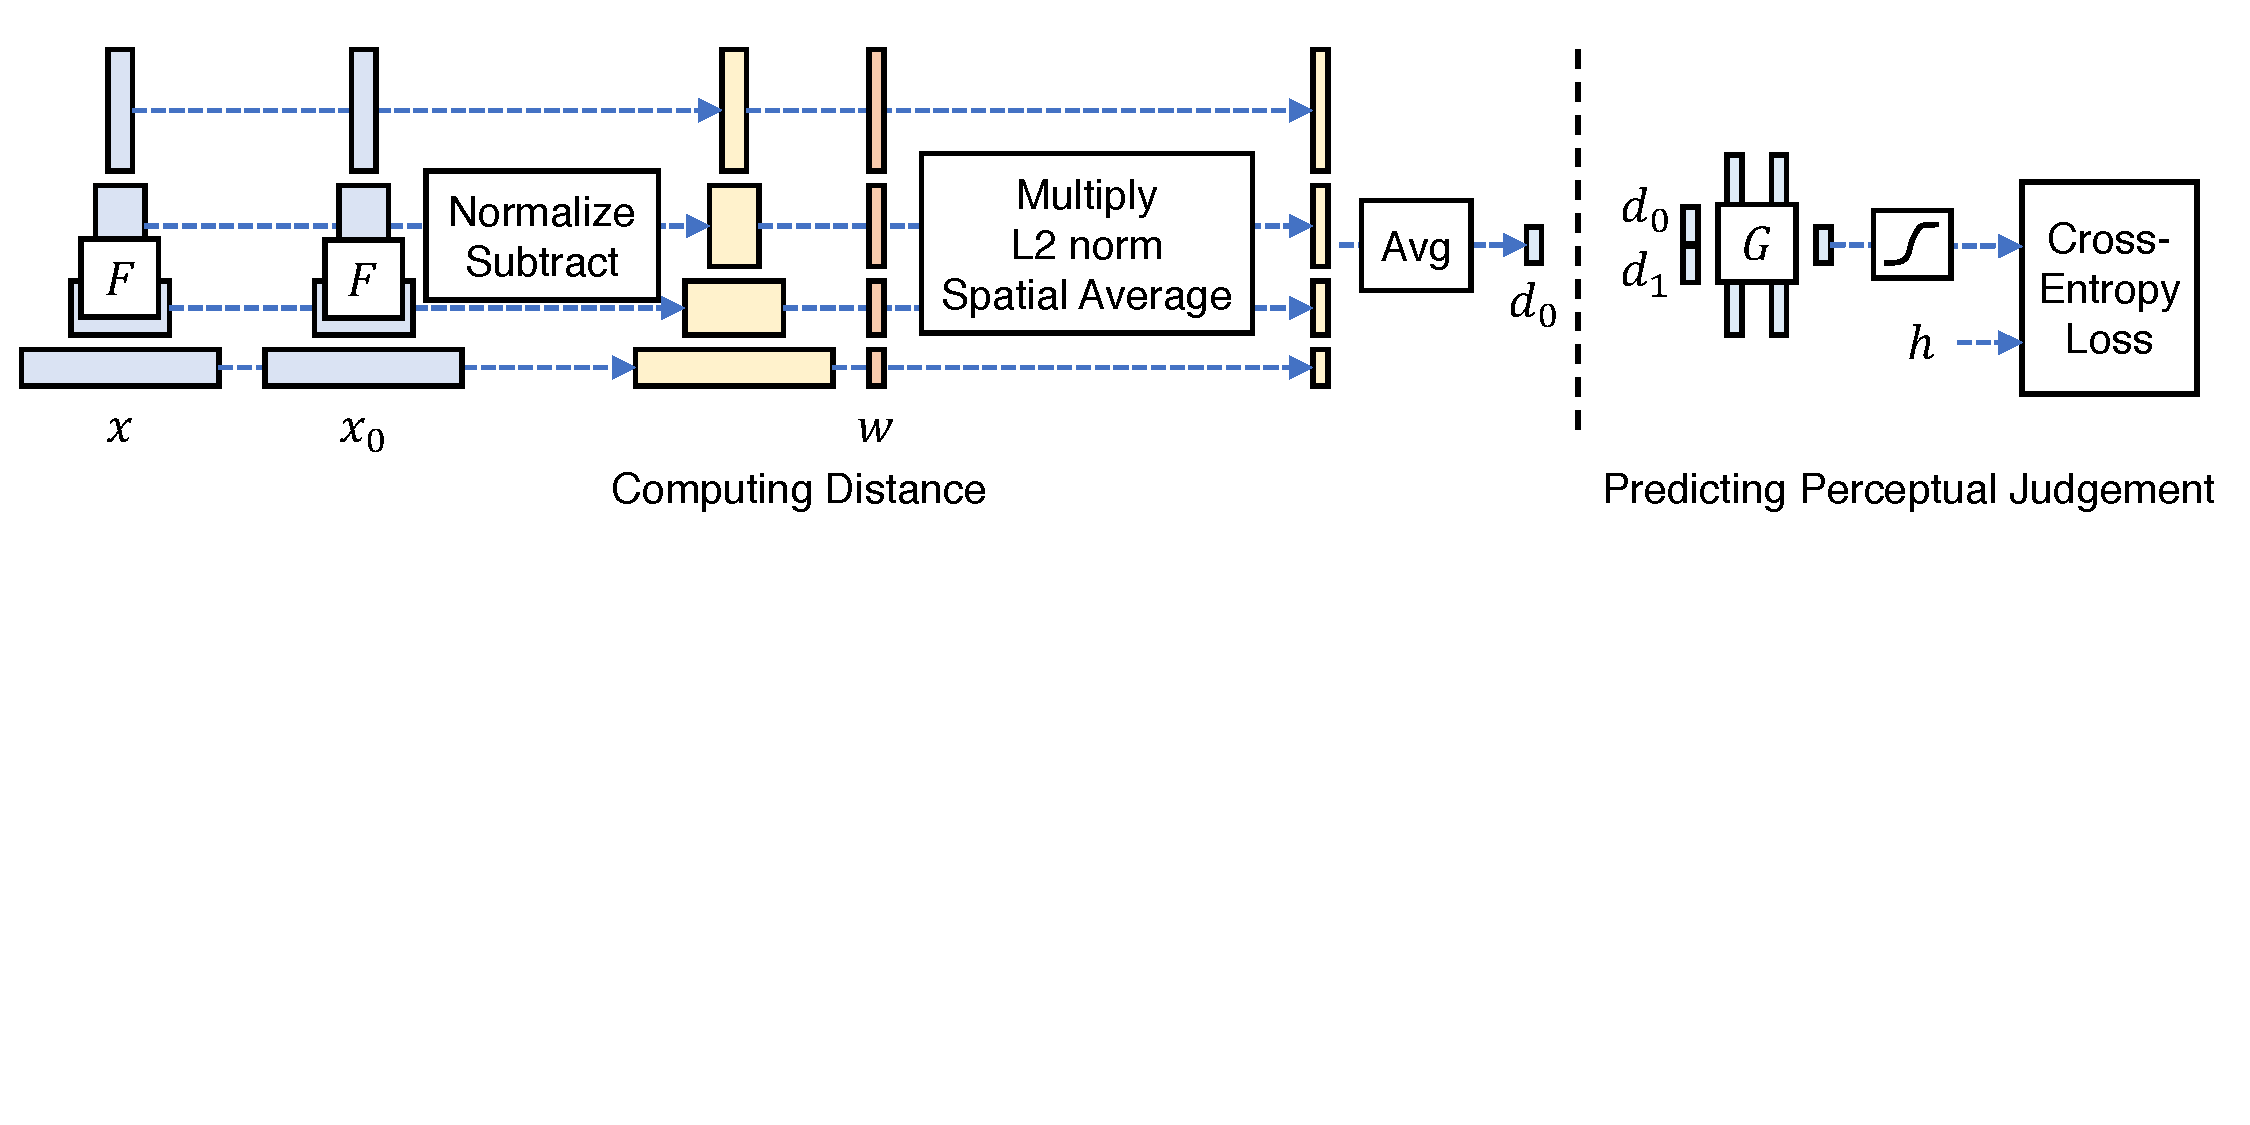
\includegraphics[width=1.0\linewidth]{imgs/network.pdf}
\vspace{-6mm}
\caption{\textbf{Computing distance from a network} (Left) To compute a distance $d_0$ between two patches, $x$, $x_0$, given a network $\mathcal{F}$, we first compute deep embeddings, normalize the activations in the channel dimension, scale each channel by vector $w$, and take the $\ell_2$ distance. We then average across spatial dimension and across all layers. (Right) A small network $\mathcal{G}$ is trained to predict perceptual judgment $h$ from distance pair ($d_0,d_1$).}
\label{fig:network}
\vspace{-1mm}
\end{figure*}

\subfile{tables/quant}

\section{Deep Feature Spaces}

We evaluate feature distances in different networks. For a given convolutional layer, we compute cosine distance (in the channel dimension) and average across spatial dimensions and layers of the network. We also discuss how to tune an existing network on our data.

\paragraph{Network architectures} We evaluate the SqueezeNet~\cite{iandola2016squeezenet}, AlexNet~\cite{krizhevsky2012imagenet}, and VGG~\cite{simonyan2014very} architectures. We use 5 \texttt{conv} layers from the VGG network, which has become the de facto standard for image generation tasks~\cite{gatys2016image,dosovitskiy2016generating,chen2017photographic}.
We also compare against the shallower AlexNet network, which may more closely match the architecture of the human visual cortex~\cite{yamins2016using}. 
We use the \texttt{conv1}-\texttt{conv5} layers from~\cite{krizhevsky2014one}. Finally, the SqueezeNet architecture was designed to be extremely lightweight ($2.8$ MB) in size, with similar classification performance to AlexNet. We use the first \texttt{conv} layer and some subsequent ``\texttt{fire}" modules.

We additionally evaluate self-supervised methods, including puzzle-solving~\cite{noroozi2016unsupervised}, cross-channel prediction~\cite{zhang2016colorful,zhang2017split}, learning from video~\cite{pathak2017learning}, and generative modeling~\cite{donahue2016adversarial}. We use publicly available networks from these and other methods, which use variants of AlexNet~\cite{krizhevsky2012imagenet}.

\paragraph{Network activations to distance} Figure \ref{fig:network} (left) and Equation~\ref{eqn:dist} illustrate how we obtain the distance between reference and distorted patches ${x,x_0}$ with network $\mathcal{F}$. We extract feature stack from $L$ layers and unit-normalize in the channel dimension, which we designate as $\hat{y}^l, \hat{y}_0^l \in \mathds{R}^{H_l\times W_l\times C_l}$ for layer $l$. We scale the activations channel-wise by vector $w^l \in \mathds{R}^{C_l}$ and compute the $\ell_2$ distance. Finally, we average spatially and sum channel-wise. Note that using $w_l=1 \forall l$ is equivalent to computing cosine distance.

\vspace{-4mm}
\begin{equation}
d(x,x_0) = \sum_l \dfrac{1}{H_l W_l} \sum_{h,w} || w_l \odot ( \hat{y}_{hw}^l - \hat{y}_{0hw}^l ) ||_2^2
\label{eqn:dist}
\end{equation}

\vspace{-2mm}

\paragraph{Training on our data} We consider a few variants for training with our perceptual judgments: \tbfit{lin}, \tbfit{tune}, and \tbfit{scratch}. For the \tbfit{lin} configuration, we keep pre-trained network weights $\mathcal{F}$ fixed, and learn linear weights $w$ on top. This constitutes a ``perceptual calibration" of a few parameters in an existing feature space. 
For example, for the VGG network, 1472 parameters are learned. For the \tbfit{tune} configuration, we initialize from a pre-trained classification model, and allow all the weights for network $\mathcal{F}$ to be fine-tuned. Finally, for \tbfit{scratch}, we initialize the network from random Gaussian weights and train it entirely on our judgments. Overall, we refer to these as variants of our proposed \textbf{Learned Perceptual Image Patch Similarity (LPIPS)} metric. We illustrate the training loss function in Figure~\ref{fig:network} (right) and describe it further in the appendix.
